\documentclass[12pt]{article}

% PACKAGES

% \usepackage[siunitx]{circuitikz}
% \usepackage{pgfornament}
% \usepackage{fancyvrb}
\usepackage[
top=2.50cm,
bottom=2.50cm,
left=2cm,
right=2cm,
marginparsep=0pt,
marginparwidth=0pt]{geometry}
\usepackage{fancyhdr}
\usepackage{float}
\usepackage{dirtree}
\usepackage{cancel}
\usepackage{mathtools}
\usepackage{amsmath}
\usepackage{amsthm}
\usepackage{amssymb}
\usepackage{textcomp}
\usepackage{ulem}
\usepackage{verbatim}
\usepackage{contour}
\usepackage{graphicx}
\usepackage{svg}
\usepackage{xcolor}
\usepackage[T1]{fontenc}
\usepackage{inputenc}
\usepackage[utf8]{inputenx}
\usepackage[unicode]{hyperref}
\usepackage[shortlabels]{enumitem}
\usepackage{booktabs}
\usepackage{bookmark}
\usepackage{listings}
\usepackage{xcolor}
\usepackage{tocloft}
\usepackage{tikz}
\usepackage[backend=biber]{biblatex}

% MACROS & DEFS

\newcommand{\floor}[1]{\left\lfloor #1 \right\rfloor}
\newcommand{\ceil}[1]{\left\lceil #1 \right\rceil}
\newcommand{\round}[1]{\left\lfloor #1 \right\rceil}
\newcommand{\abs}[1]{\left\lvert #1 \right\rvert}

\DeclareRobustCommand{\ul}[1]{%
	\uline{\phantom{#1}}%
	\llap{\contour{white}{#1}}%
}

\renewcommand{\ULdepth}{1.8pt}
\contourlength{0.8pt}

\setlength{\parindent}{0em}
\setlength{\parskip}{0.75em}

\definecolor{codegreen}{RGB}{0,135,0}
\definecolor{codegray}{RGB}{135,135,135}
\definecolor{codemagenta}{RGB}{215,0,135}
\definecolor{codepurple}{RGB}{135,0,175}
\definecolor{backcolour}{RGB}{238,238,238}

% PACKAGE CONFIG

% \usetikzlibrary{calc, arrows, positioning, circuits.logic.US}
\graphicspath{ {./images/} }

% Biblography
% \addbibresource{dsa.bib}

\lstdefinestyle{code}{
	basicstyle=\ttfamily\small,
	commentstyle=\color{codegray}\itshape,
	keywordstyle=\color{codepurple},
	stringstyle=\color{codegreen},
	aboveskip=15pt,
	captionpos=b,
	abovecaptionskip=12.5pt,
	breaklines=true,
	numbers=none,
	frame=tb,
	framesep=5pt,
	keepspaces=true,
	showspaces=false,
	showstringspaces=false,
	breakatwhitespace=false,
	tabsize=2,
	showtabs=false,
}

\lstset{style=code}

% Set dots for table of contents
\renewcommand{\cftdot}{.}
\renewcommand{\cftsecleader}{\cftdotfill{\cftdotsep}}

% Set theorem
\newtheorem*{definition}{Definition}

% HEADER & FOOTER

\setlength{\headheight}{15pt}
\pagestyle{fancy}
\renewcommand{\headrulewidth}{0pt}
\lhead{J. Scerri}
\chead{CPS1012 --- Coursework}
\rhead{\thepage}

% TITLE

\title{CPS1012 --- Operating Systems \& Systems Programming 1\\
\vspace{1em}\textbf{Coursework}}

\date{\today}

\author {{\textbf{Juan Scerri}}\\
B.Sc. (Hons)(Melit.) Computing Science and Mathematics (First Year)}

\begin{document}

%----------------------------------
%	TITLE PAGE
%----------------------------------

\maketitle % Print the title page

\thispagestyle{empty} % Suppress headers and footers on the title page

%----------------------------------

\tableofcontents

\clearpage

\lstlistoflistings

\clearpage

\section{Plagiarism Declaration}

Plagiarism is defined as \textit{``the unacknowledged use, as
one's own, of work of another person, whether or not such work
has been published, and as may be further elaborated in Faculty
or University guidelines''} (\ul{University Assessment
Regulations}, 2009, Regulation 39 (b)(i), University of Malta).

I, the undersigned, declare that the report submitted is my
work, except where acknowledged and referenced. I understand
that the penalties for committing a breach of the regulations
include loss of marks; cancellation of examination results;
enforced suspension of studies; or expulsion from the degree
programme.

Work submitted without this signed declaration will not be
corrected, and will be given zero marks.

\vfill

\begin{minipage}[t]{0.3\textwidth}
\ul{Juan Scerri} \medskip

\textbf{Student's full name} \medskip
\end{minipage}
\hfill
\begin{minipage}[t]{0.3\textwidth}
\ul{CPS1012} \medskip

\textbf{Study-unit code} \medskip
\end{minipage}
\hfill
\begin{minipage}[t]{0.3\textwidth}
\ul{{\today}} \medskip

\textbf{Date of submission} \medskip
\end{minipage}

\vspace{2cm}

\textbf{Title of submitted work:} \ul{Operating Systems \&
Systems Programming 1 Coursework}

\vspace{2cm}

\textbf{Student's signature} \medskip

\underline{
\includegraphics[height=2cm]{sig}} \medskip

\section{Structure \& Design}

\subsection{Structure}

The coursework was broken up into four tasks.

All the questions of \textit{Task 1} have been answered
separately, each having there own \texttt{.c} file.

The two questions of \textit{Task 2} where answered in one
\texttt{.c} file.

\textit{Task 3} and \textit{Task 4} where done simultaneously to
avoid code repetition and reduce complexity of development. This
is because it is easier to develop an interpreter where all the
constraints are known.

Naturally, some of the code developed from \textit{Task 1} and
\textit{Task 2} was copied over to the directory of \textit{Task
3} and \textit{Task 4}. Specifically, the relevant code from
\textit{Task 1} was placed in \texttt{external.c} and the
relevant code from \textit{Task 2} was placed in
\texttt{builtin.c}.

\textit{Note:} There is an extra directory called \texttt{util}
which contains older versions of code which can be found in
\texttt{interpreter.c}. The header files within this directory
are used in \textit{Task 1} and \textit{Task 2} to allow for
easier testing.

\begin{center}
\begin{minipage}[t]{0.3\textwidth}
\dirtree{%
.1 /.
.2 src.
.3 task1.
.3 task2.
.3 task3and4.
.3 util.
.3 .clang-format.
.3 CMakeLists.txt.
.2 .clang-format.
.2 .gitignore.
.2 README.md.
}
\end{minipage}
\begin{minipage}[t]{0.3\textwidth}
\dirtree{%
.1 util.
.2 .clang-format.
.2 linenoise.c.
.2 linenoise.h.
.2 peek\_stream.c.
.2 peek\_stream.h.
.2 string\_vec.c.
.2 string\_vec.h.
.2 tokeniser.c.
.2 tokeniser.h.
.2 util.h.
}
\end{minipage}
\end{center}

\begin{center}
\begin{minipage}[t]{0.3\textwidth}
\dirtree{%
.1 task1.
.2 .clang-format.
.2 qa.c.
.2 qb.c.
.2 qc.c.
.2 qd.c.
.2 qe.c.
}
\end{minipage}
\begin{minipage}[t]{0.3\textwidth}
\dirtree{%
.1 task2.
.2 .clang-format.
.2 qab.c.
}
\end{minipage}
\begin{minipage}[t]{0.3\textwidth}
\dirtree{%
.1 task3and4.
.2 .clang-format.
.2 builtin.c.
.2 builtin.h.
.2 external.c.
.2 external.h.
.2 interpreter.c.
.2 interpreter.h.
.2 linenoise.c.
.2 linenoise.h.
.2 tests.txt.
.2 tish.c.
}
\end{minipage}
\end{center}

\subsection{Design}

In this section the majority of the implemented algorithms and
design will be explained through diagrams/images. Where
necessary supplementary explanation will be provided and codes
snippets will be inserted.

\subsubsection{Design of Task 1}

\begin{figure}[H]
\centering
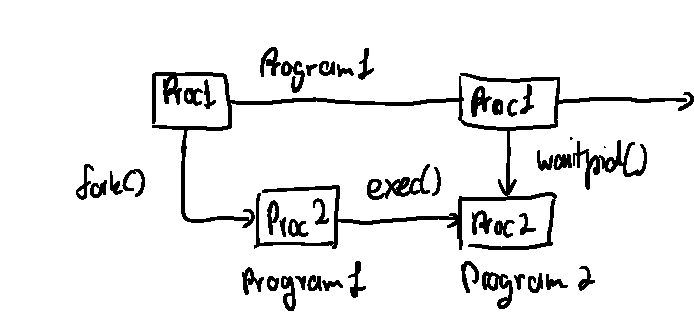
\includegraphics[height=4.5cm]{task1qa}
\caption{A drawing of the \texttt{fork-exec-wait} pattern.}
\end{figure}

For question (a), the requested algorithm implements a simple
\texttt{fork-exec-wait} pattern. This pattern is used to allow
processes to load other programs.

Nevertheless, this might not always be enough. If two or more
processes need to communicate with each other, they need to make
use of Inter-Process Communication (IPC) mechanisms. For
question (b), two processes will be allowed to communicate
together through a \ul{pipe} an OS provided IPC mechanism.

\textit{Note:} Configuration of the pipes is done after
\texttt{fork()} and before \texttt{exec()}.

\lstinputlisting[caption={Configuration after \texttt{fork()}
and before \texttt{execvp()}.},language=C, firstline=37,
lastline=47]{src/task1/qb.c}

\begin{figure}[H]
\centering
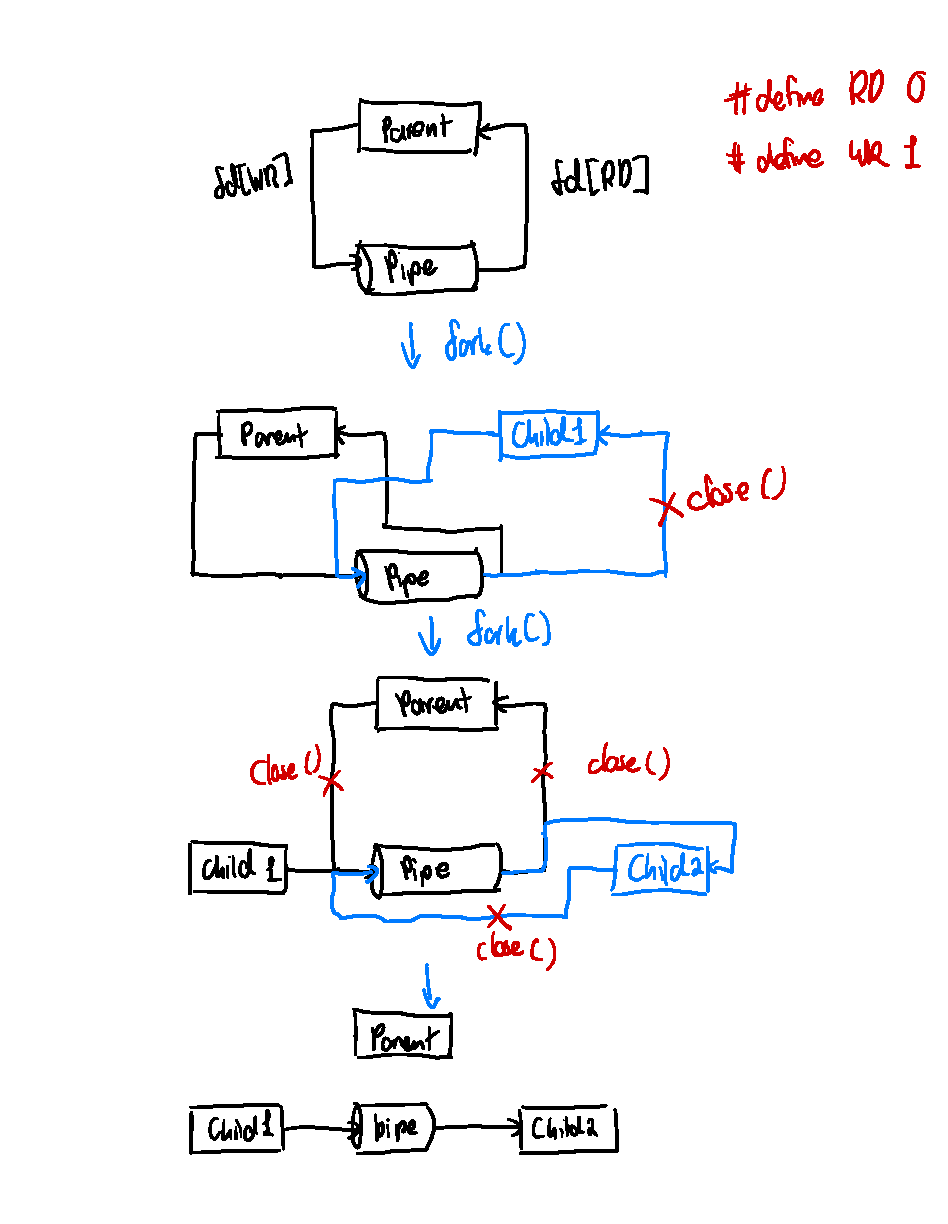
\includegraphics{task1qb}
\caption{A drawing of the procedure used to connect two processes
through a pipe.}
\end{figure}

\begin{figure}[H]
\centering
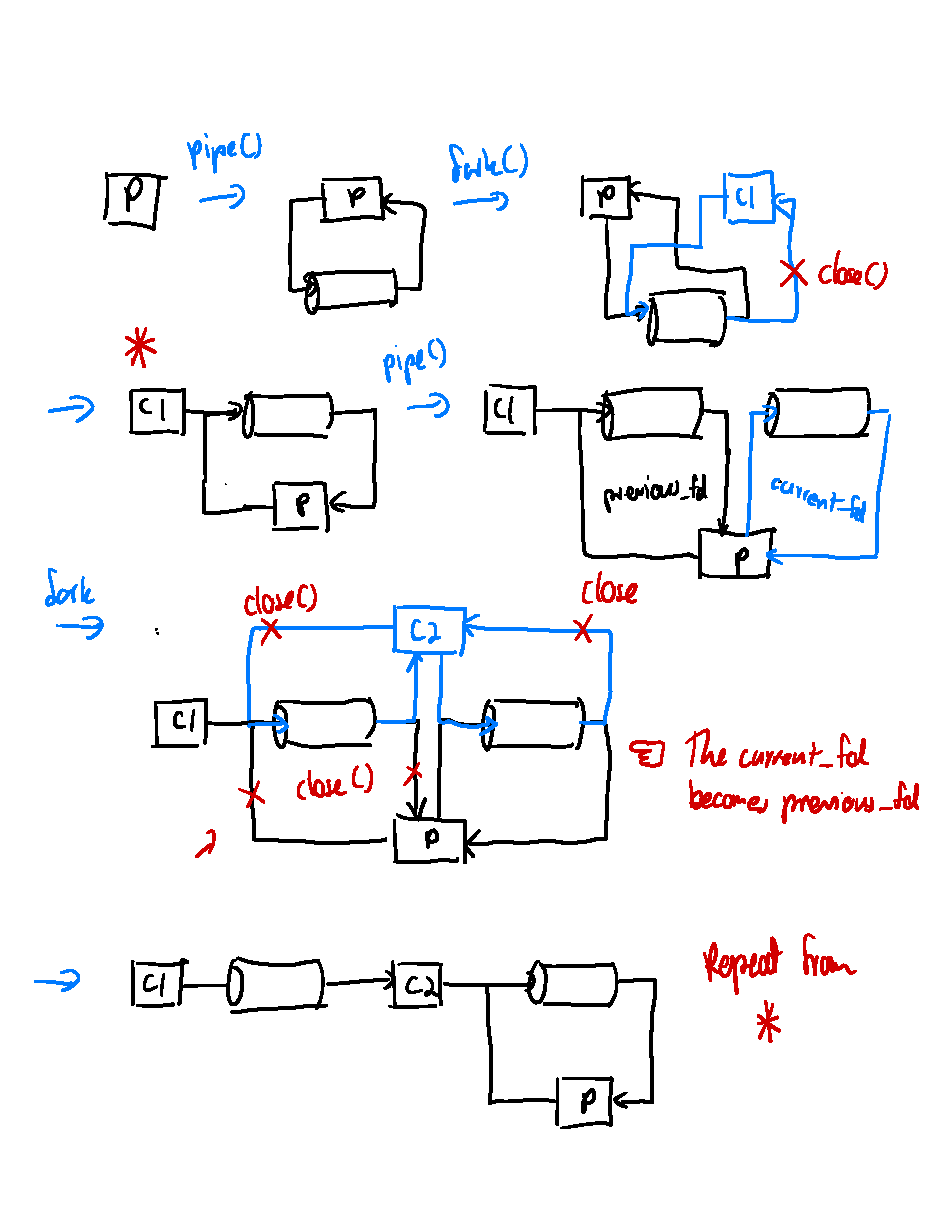
\includegraphics{task1qc1}
\caption{A drawing of the start procedure and intermediate
procedure used to construct a pipeline.}
\label{gen_pipeline}
\end{figure}

\newpage

For question (c), a new variant was created called
\texttt{execute\_pipeline()}. As input, it takes in a
\texttt{NULL}-terminated array of programs (of type \texttt{char
**}). Then, it constructs a \ul{pipeline} which allows every
program to communicate with the next program in the array. This
is done through the procedure described in figure
\ref{gen_pipeline}.

\textit{Note:} There is no need to know the length of the
pipeline. This is because the only four file descriptors which
the parent has awareness of at any one point in time during the
construction of the pipeline, are the file descriptors 
associated with the previous and current pipe.

\begin{figure}[H]
\centering
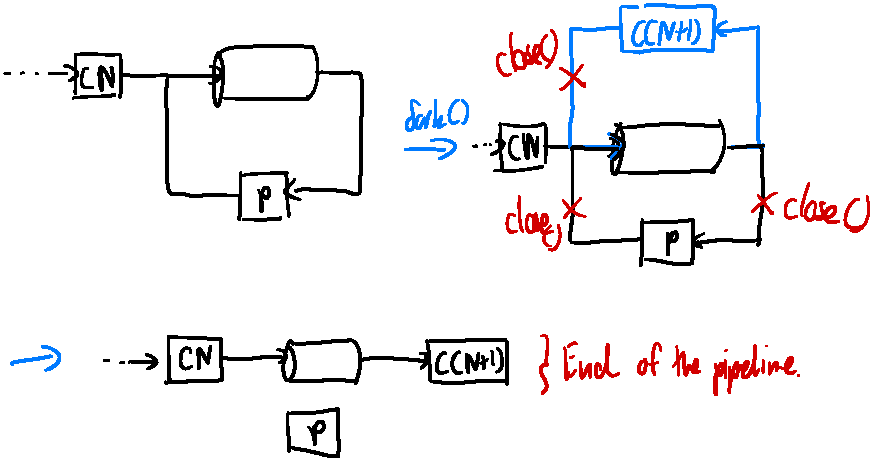
\includegraphics{task1qc2}
\caption{A drawing of the end procedure used to construct a
pipeline.}
\label{end_pipeline}
\end{figure}

In particular there are three distinct unique procedures which
the algorithm has to perform. These are labelled as \ul{start},
\ul{intermediate} (described in figure \ref{gen_pipeline}) and
\ul{end} (described in figure \ref{end_pipeline}). In particular
the intermediate step is repeated until the end is reached.

\lstinputlisting[caption={\texttt{waitpid()} being called in the
parent for every forked process.},language=C, firstline=80,
lastline=89]{src/task1/qd.c}

\newpage

For question (d), an \texttt{options} parameter was added to the
previous function and a call to \texttt{waitpid()} is made for
every forked process (see the above listing).

The function blocks for every process to ensure no zombie
processes are present. Figure \ref{zombies} demonstrates a
version of the question where the function blocks only for
the last process.

\begin{figure}[H]
\centering
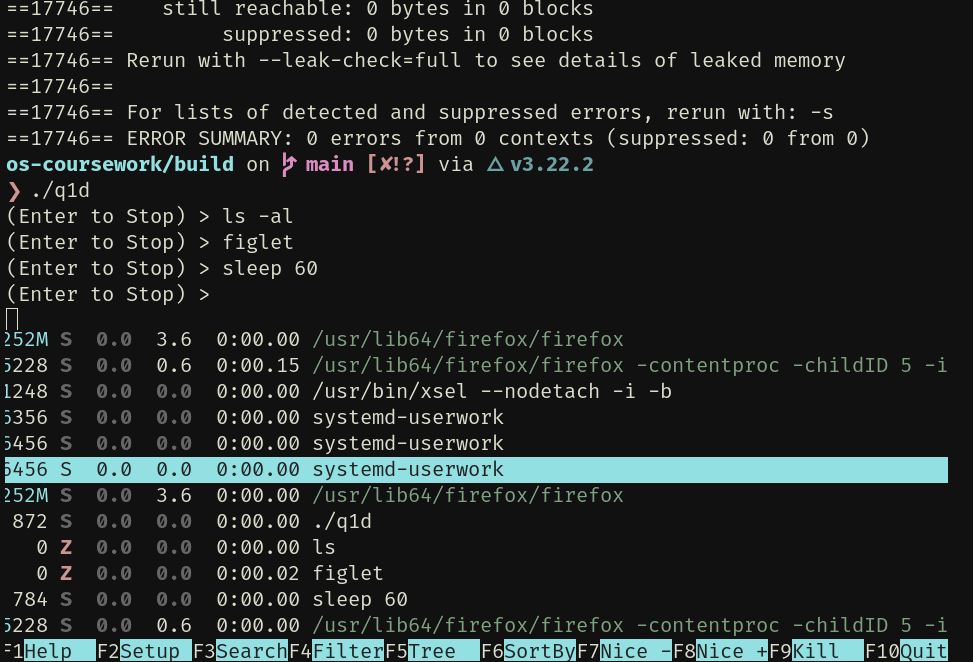
\includegraphics[width=12cm]{zombies}
\caption{A screenshot of zombie processes (in \texttt{htop})
present because the function waits only for the last process.}
\label{zombies}
\end{figure}

\lstinputlisting[caption={Redirecting pipeline
input.},language=C, firstline=95, lastline=99]{src/task1/qe.c}

\lstinputlisting[caption={Redirecting pipeline
output.},language=C, firstline=123, lastline=129]{src/task1/qe.c}

For question (e), a simple addition of three extra parameters and
two if-statements in the start and end steps suffice to redirect
the input and the output of the pipe. The third parameter is a
flag used to choose between appending to a file or truncating a
file.

\subsubsection{Design of Task 2}

For question (a), the structure of what needs to be implemented is
laid out clearly in the question. Specifically, the creation of
a structure for holding function pointers and function names
together. 

Then a linear search is performed every time before trying to
execute an external process to check if the specified command is
a builtin.

For question (b) a number of builtin functions had to be
implemented.

\texttt{sh\_exit()} is the simplest of the functions simply
calling the \texttt{exit()} function from \texttt{stdlib.h}.

\texttt{sh\_ver()} prints a formatted string to \texttt{stdout}
containing the author's name, version and a small message. The
author's name, version and message are all \texttt{\#define}s.

\lstinputlisting[caption={The declaration of the global
\texttt{cwd}.},language=C, firstline=10,
lastline=16]{src/task2/qab.c}

\lstinputlisting[caption={Initialising
\texttt{cwd}.},language=C, firstline=114,
lastline=117]{src/task2/qab.c}

\texttt{sh\_cwd()} prints the contents of the global variable
\texttt{cwd} to \texttt{stdout}. \texttt{cwd} is a character
array with a length of \texttt{PATH\_MAX}, which is a definition
found in \texttt{linux/limits.h} on Linux. If the OS is not
Linux, the limit will be set to 4096 characters. Moreover, the
global has to be initialised at the start of the shell.

\texttt{sh\_cd()} uses \texttt{chdir()} to change the current
directory of the shell to the first argument provided to
\texttt{cd} or to the home directory of the current user if no
argument is provided. Naturally, \texttt{sh\_cd()} will have to
update \texttt{cwd} every time since the directory might change.

\subsubsection{Design of Task 3 and 4}

\begin{figure}[H]
\centering
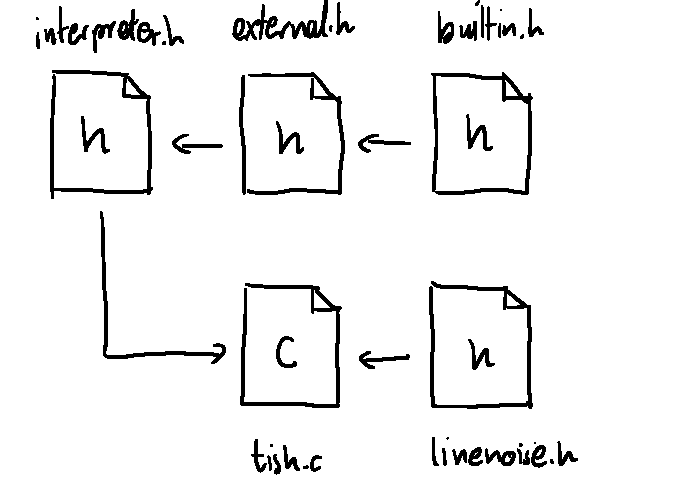
\includegraphics{task3arch}
\caption{A drawing of how the files used for \textit{Task 3} and
\textit{Task 4} are linked (through \texttt{\#include}).}
\end{figure}

The design of these tasks have been merged into one.
Particularly, there are five main \texttt{.c} files.
\texttt{external.c} contains the functions written for
\textit{Task 1} and \texttt{builtin.c} contains the functions
written for \textit{Task 2}. \texttt{interpreter.c} is the file
where all the new functionality is present. Specifically, it
contains, the tokeniser, syntactic checker and translator.
Moreover, it also contains a simple \texttt{execute()} function
which interacts with the components in \texttt{external.c} and
\texttt{builtin.c} through the header files.

\texttt{linenoise.c} is the suggest line editing library, which
allows for the easy creation of prompts and command line user
interfaces. The repository of the original author can be found
at \url{https://github.com/antirez/linenoise}.

\texttt{tish.c} is the source file which brings all of these
components together to create a functional shell named `Tiny
Shell' (\texttt{tish}).

\begin{figure}[H]
\centering
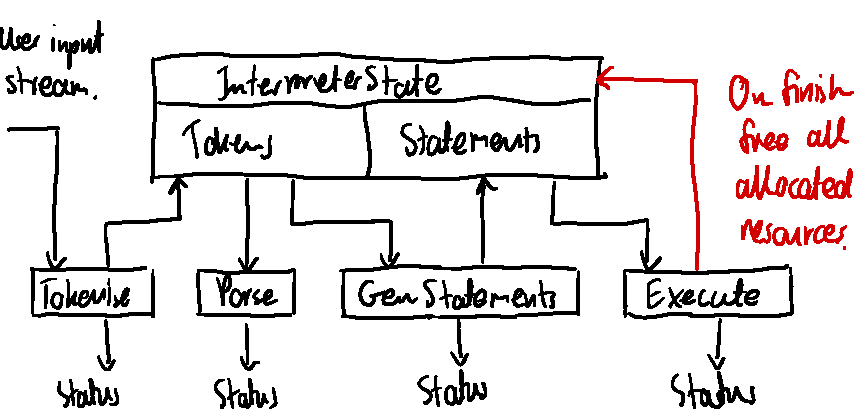
\includegraphics{interpreter-arch}
\caption{A drawing of how the interpreter is structured and how
it processes user input lines.}
\end{figure}

In the interpreter there is one static global structure which is
used throughout all of the components of the interpreter. These
components/functions are the following: \texttt{tokenise()},
\texttt{parse()}, \texttt{genStatements()} and
\texttt{execute()}. There is one exposed function in the file
\texttt{interpret()} and it is called in \texttt{tish.c}.

\begin{figure}[H]
\centering
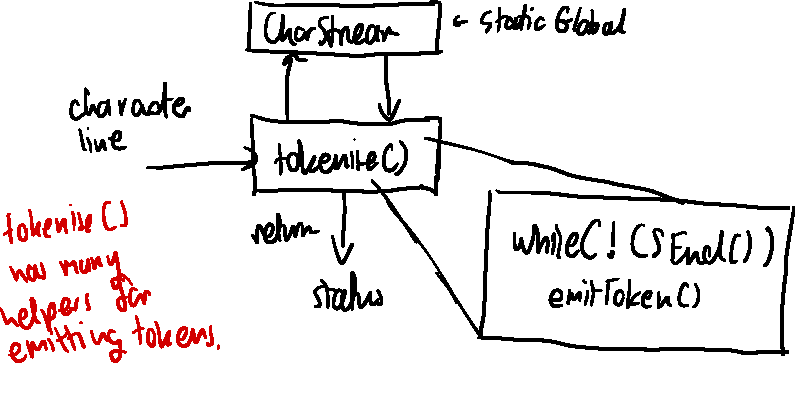
\includegraphics{tokeniser}
\caption{This is a simple description of how the
tokeniser works.}
\end{figure}

The \texttt{tokenise()} function makes use of a static global
called \texttt{CharStream}. This allows the tokeniser to
traverse a character array without losing state across different
function calls. This makes the code more readable and
manageable.

The most important functions in the tokeniser are the emitters.
They basically emit a token which can later be used to check if
the user input is syntactically correct. Emitted tokens are
stored in the interpreter state. Escaping of characters is dealt
with in two emitters: \texttt{emitString()} and
\texttt{emitQuotedString()}.

\begin{figure}[H]
\centering
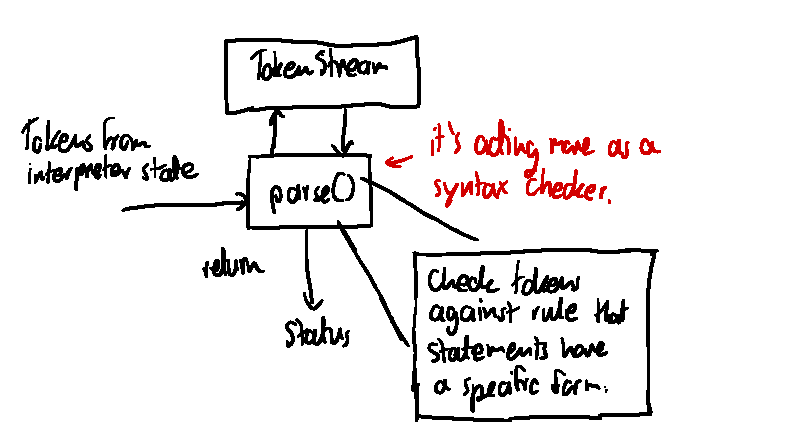
\includegraphics{parser}
\caption{this is a simple description of how the
parser works.}
\end{figure}

\texttt{parse()} initialises the \texttt{TokenStream} and checks
if syntax of the tokens is correct. The general form of a
statement is:

\begin{verbatim}
statement := cmd1 | cmd2 | ... | cmdN  < infile {> / >>} outfile
cmd := prg arg1 arg2 ... argN
prg := str
arg := str
\end{verbatim}

If a collection of tokens cannot fit into the above
production rule, the parser will print an error and clean any
allocated resources.

\textit{Note:} Many of the characters are optional for example
there is no need for input or/and output redirection.
Nevertheless, if for example a \texttt{>} is present it must be
followed by the \texttt{infile}. In the function there are many
similar rules.

After checking that the tokens are syntactically correct, other
functions specifically \texttt{genStatements()} can assume a lot
about the structure of the tokens. The \texttt{genStatements()}
function does two main things. It counts the number of commands
in a pipeline and the number of strings per command.

Having this information allows the function to allocate the
exact amount of memory required for the statements which are
then populated accordingly.

\textit{Note:} The process of counting, allocating and
populating are all done simultaneously throughout the code. This
is because it is more convenient for certain tasks to be done
when the information is directly available.

The \texttt{execute()} function has two parts. The first part
checks if the command is a builtin. If the command is a builtin
\texttt{execute()} will call the respective builtin function.
Otherwise, it will try to execute an external program.

\textit{Note:} There are two scenarios where -2, which is
defined as \texttt{EXIT\_SHELL}, is returned. First, when the
\texttt{exit()} builtin is called or second, when a forked
process fails. The latter case is special because it avoids the
possibility of having two concurrent shell processes where the
forked shell spins because its \texttt{stdin} is bound to a
pipe.

The final function is \texttt{interpret()} and it collects all
of these functions together into one function which can be
called in \texttt{tish.c}. Specifically, in \texttt{tish.c}
there is an event loop which waits for user input and then
passes the user input to \texttt{interpret()} and the process
repeats until the user decides to exit.

\section{Testing Methodology}

\subsection{Testing for Task 1}

\begin{figure}[H]
\centering
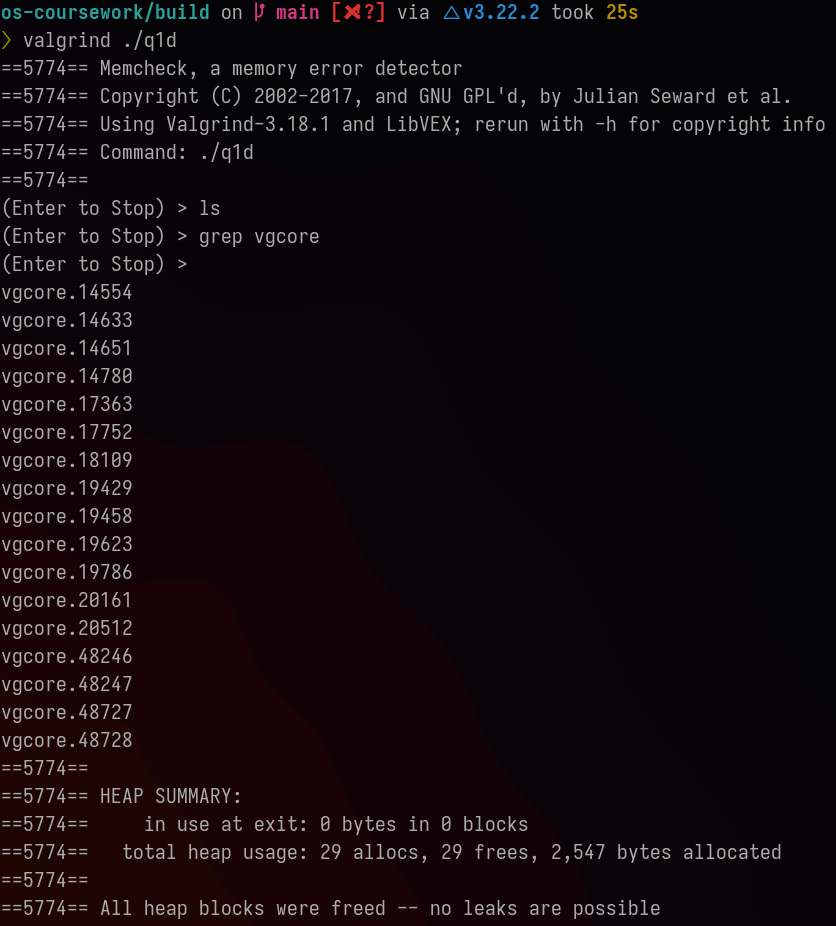
\includegraphics[width=11cm]{q1d-test}
\caption{A screenshot of the \texttt{q1d} executable running
under \texttt{valgrind}.}
\end{figure}

For testing, all functions developed in \textit{Task 1} were
isolated in there own file, with a simple main function.

The main function contains a simple prompt which allows for
user input. Commands where entered and the output was noted and
compared to the expected behaviour.

Moreover, \texttt{valgrind} was used to make sure that no memory
was being leaked and no errors where being report. Moreover, all
compiler warnings were enabled (see the \texttt{CMakeLists.txt}
file).

\textit{Note:} To properly test for blocking, a command like
\texttt{sleep 10} was used (see figure \ref{zombies}). Moreover,
testing of the answer for question (e) was done with hard coded
file names (see functions \texttt{test1()} and \texttt{test2()}
in \texttt{src/task1/qe.c}).

\subsection{Testing for Task 2}

\begin{figure}[H]
\centering
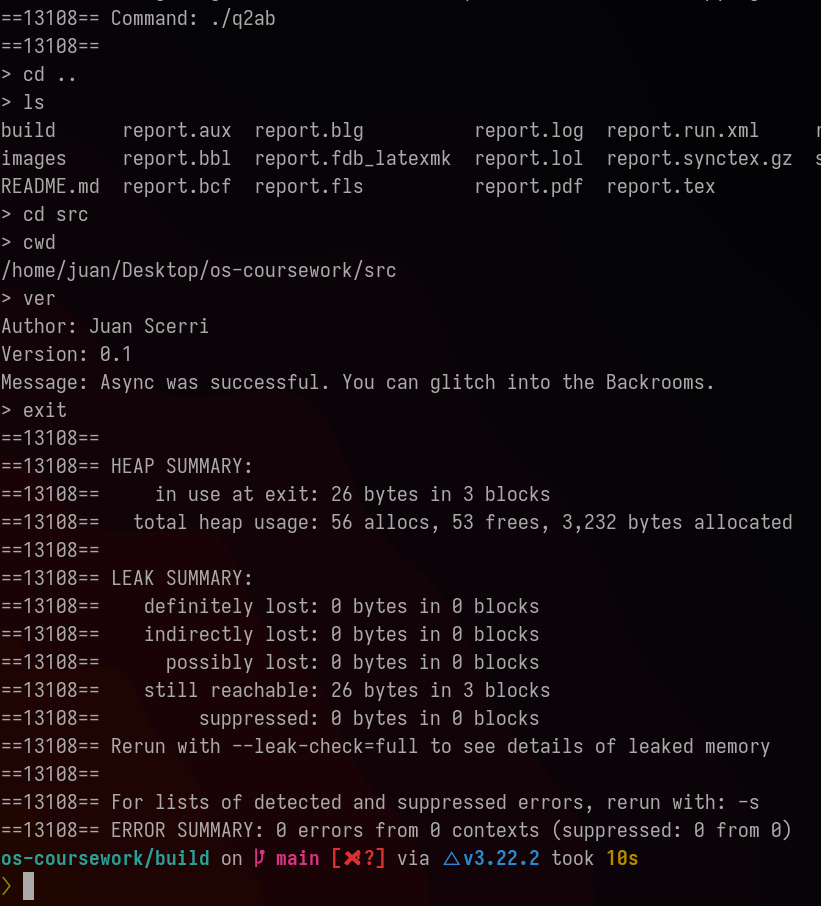
\includegraphics[width=12cm]{q2ab-test}
\caption{A screenshot of the \texttt{q2ab} executable running
under \texttt{valgrind}.}
\end{figure}

Testing for \textit{Task 2} was performed using a similar method
to \textit{Task 1}.

\textit{Note:} The implementation of \texttt{exit} in this task
leaks memory because it is using \texttt{exit()} with freeing
any potentially allocated data. This has been addressed in the
actual shell.

\subsection{Testing for Task 3}

Testing for \textit{Task 3} is a bit more complicated because it
requires a lot of debug output to ensure that tokenisation,
parsing and translation into statements are being done
correctly.

\newpage

\lstinputlisting[caption={Comment indicating the usage of
\texttt{\#define DEBUG}.},language=C, firstline=8,
lastline=10]{src/task3and4/interpreter.c}

\lstinputlisting[caption={Usage of the \texttt{DEBUG} definition for
debugging.},language=C, firstline=516, lastline=518]{src/task3and4/interpreter.c}

To do this, a number of functions calls (\texttt{fprintf(stderr,
...)}) are littered throughout the code. They can be activated
by defining \texttt{DEBUG} in the \texttt{interpreter.c} source
file and recompiling.

\begin{figure}[H]
\centering
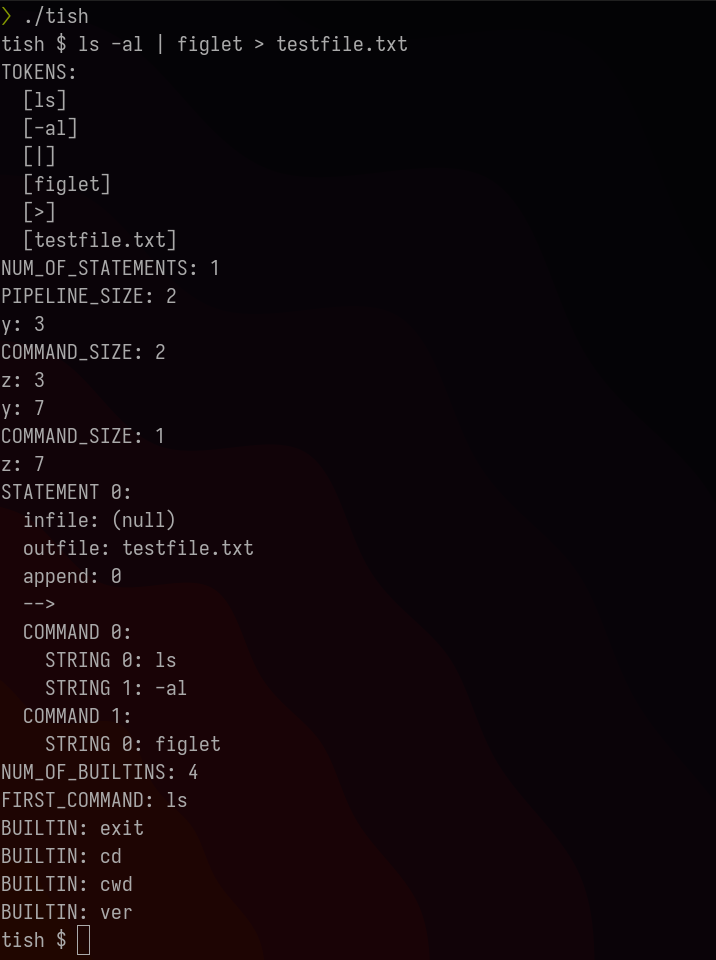
\includegraphics[width=10cm]{task3and4-test}
\caption{A screenshot of the \texttt{tish} executable running
with \texttt{DEBUG} defined.}
\end{figure}

\textit{Note:} A list of test input can be found at
\texttt{src/task3and4/test.txt}. There are ten test inputs. They
are all identified as being either valid or invalid.

\section{Issues \& Bugs}

\subsection{Issues}

There are a number off issues both with regards to the design of
the code and the functionality of the shell.

\subsubsection{Design Issues}

\begin{itemize}
\item
  The way in which the shell exits could be improved through the
  use of an exit handler.
\item
  A revamped interpreter, generating an actual Abstract Syntax
  Tree (AST) could help both readability and versatility. Along
  with allowing the shell to conform to POSIX-like behaviour.
  For example the behaviour of \texttt{bash} and \texttt{tish}
  are very different for the following command \texttt{figlet |
  sed "s/ /*/g" < infile.txt}.
\item
  The current implementation of \texttt{tish}, especially the
  interpreter relies heavily on heap-allocated memory. It would
  be beneficial if heap-allocations are reduced both for
  performance and code readability, as often times
  control flow is obscured because of constant validation and
  error checking.
\end{itemize}

\subsubsection{Functionality Issues}

\begin{itemize}
\item
  As already mentioned the current shell does not conform to a
  \texttt{bash}-like syntax. So, improving compatibility with
  already existing shells would be beneficial.
\item
  Currently, \texttt{Ctrl-C} causes the whole shell to exit even
  whilst running a program like \texttt{figlet} in
  \texttt{stdin}. This should be changed to simply kill the
  current blocking program in the shell. This could either be
  done by registering a signal handler for \texttt{SIGINT} or by
  entering into raw mode so the bytes can be handled directly.
\end{itemize}

\subsection{Bugs}

From the testing I have done, I have not found any bugs or
unexpected behaviour in the final binary i.e. \texttt{tish}.

As I mentioned throughout the document there were some minor
issues (e.g. memory leaks, zombies etc.) which where present in
the earlier versions of the code.

\end{document}
